\documentclass[class=article,border=5pt,tikz]{standalone}
\usetikzlibrary{calc}

% define a box
\tikzset{%
  box/.style={rectangle, draw=black, minimum size=1cm},
}

\usepackage{pgf}
% check if is multiple of argument
% \ifismultiple{15}{4}{true}{false}
\newcommand\ifismultiple[4]{%
    \pgfmathparse{mod(#1,#2)==0}
    \let\r\pgfmathresult
    \ifnum\r=1
        #3%
    \else
        #4%
    \fi
}

% mark all the muliples of 3, 4, 5
\newcommand{\drawmultiples}{%
    \foreach \x in {1,...,10}{
        \foreach \y in {1,...,6}{
            \pgfmathsetmacro\z{int(\x+(\y-1)*10-1)}
            \node[box,draw=black] at (\x-0.5,6-\y+0.5) {\z};
            \ifnum\z>0  % do not treat zero as a multiple
                \ifismultiple{\z}{3}{%
                  \node[box,fill=red,opacity=0.4] at (\x-0.5,6-\y+0.5){};
                }{}
                \ifismultiple{\z}{4}{%
                  \node[box,fill=blue,opacity=0.4] at (\x-0.5,6-\y+0.5){};
                }{}
                \ifismultiple{\z}{5}{%
                  \node[box,fill=green,opacity=0.4] at (\x-0.5,6-\y+0.5){};
                }{}
            \fi
        }
    }
}

\begin{document}

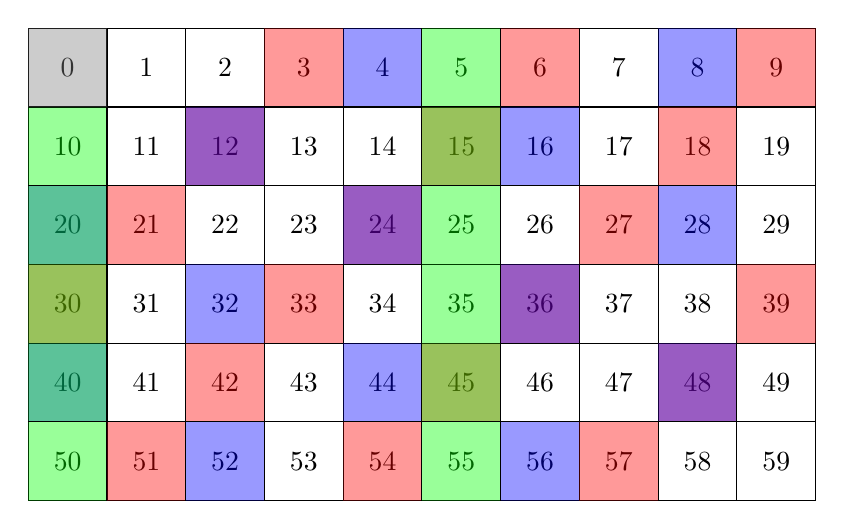
\begin{tikzpicture}
  % mark multiples of 3,4,5
  \drawmultiples
  % mark day 0
  \node[box,fill=gray,opacity=0.4] at (1-0.5,6-0.5){};
\end{tikzpicture}

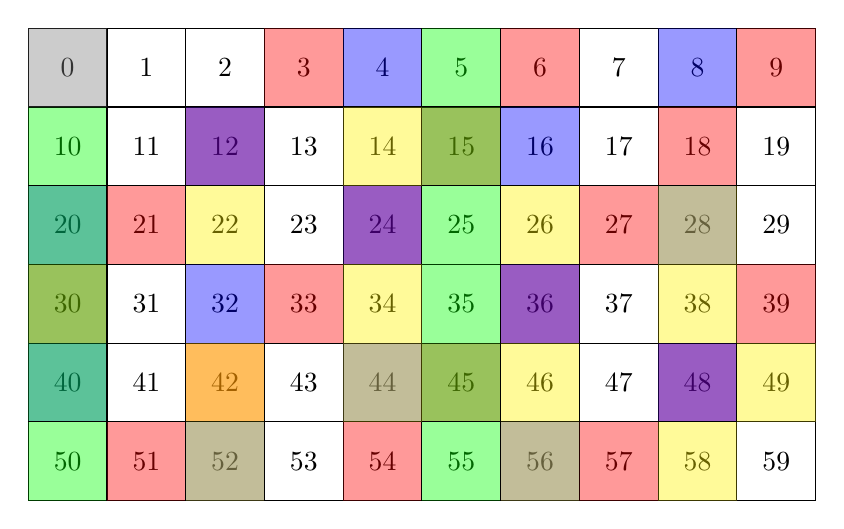
\begin{tikzpicture}
  % mark multiples of 3,4,5
  \drawmultiples
  % mark day 0
  \node[box,fill=gray,opacity=0.4] at (1-0.5,6-0.5){};
  % draw multiples of the primes
  \foreach \x in {1,...,10}{
      \foreach \y in {1,...,6}{
          \foreach \w in {14, 22, 26, 34, 38, 46, 58, 49}{
              \pgfmathsetmacro\z{int(\x+(\y-1)*10-1)}
              % ignore the zero cell
              \ifnum\z>0
                \ifismultiple{\z}{\w}{%
                    \node[box,fill=yellow,opacity=0.4] at (\x-0.5,6-\y+0.5) {};
                }{}
              \fi
          }
      }
  }
\end{tikzpicture}

\end{document}
